\chapter{Figures from the NVidia Programming Guide}

Figures~\ref{fig:gpu-devotes-more-transistors-to-data-processing}, \ref{fig:floating-point-operations-per-second}, \ref{fig:memory-bandwidth} are provided by the NVidia CUDA Programming Guide \cite{CudaGuide2013}

\begin{figure}
\centering
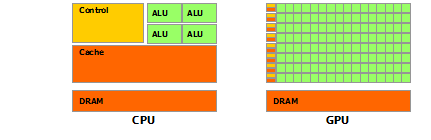
\includegraphics[width=0.9\textwidth]{gpu_content/nvidia_figures/gpu-devotes-more-transistors-to-data-processing.png}
\caption{The GPU Devotes More Transistors to Data Processing (Image courtesy of NVidia \cite{CudaGuide2013})} 
\label{fig:gpu-devotes-more-transistors-to-data-processing}
\end{figure}

\begin{figure}
\centering
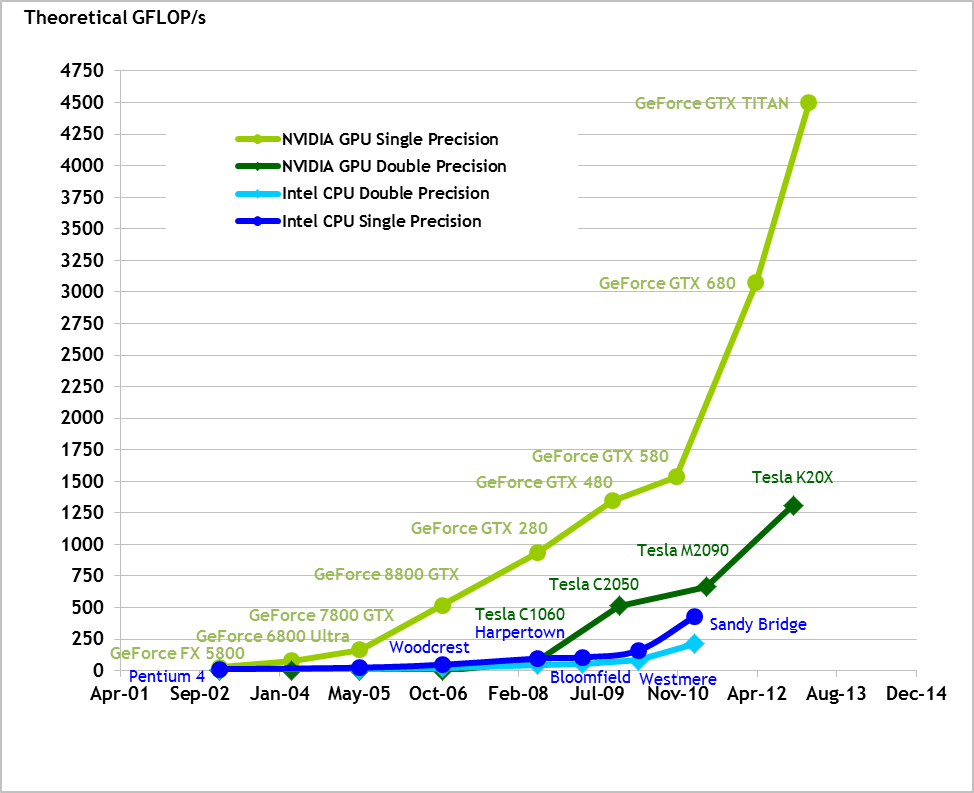
\includegraphics[width=0.9\textwidth]{gpu_content/nvidia_figures/floating-point-operations-per-second.png}
\caption{Floating-Point Operations per Second for the CPU and GPU (Image courtesy of NVidia \cite{CudaGuide2013})} 
\label{fig:floating-point-operations-per-second}
\end{figure}

\begin{figure}
\centering
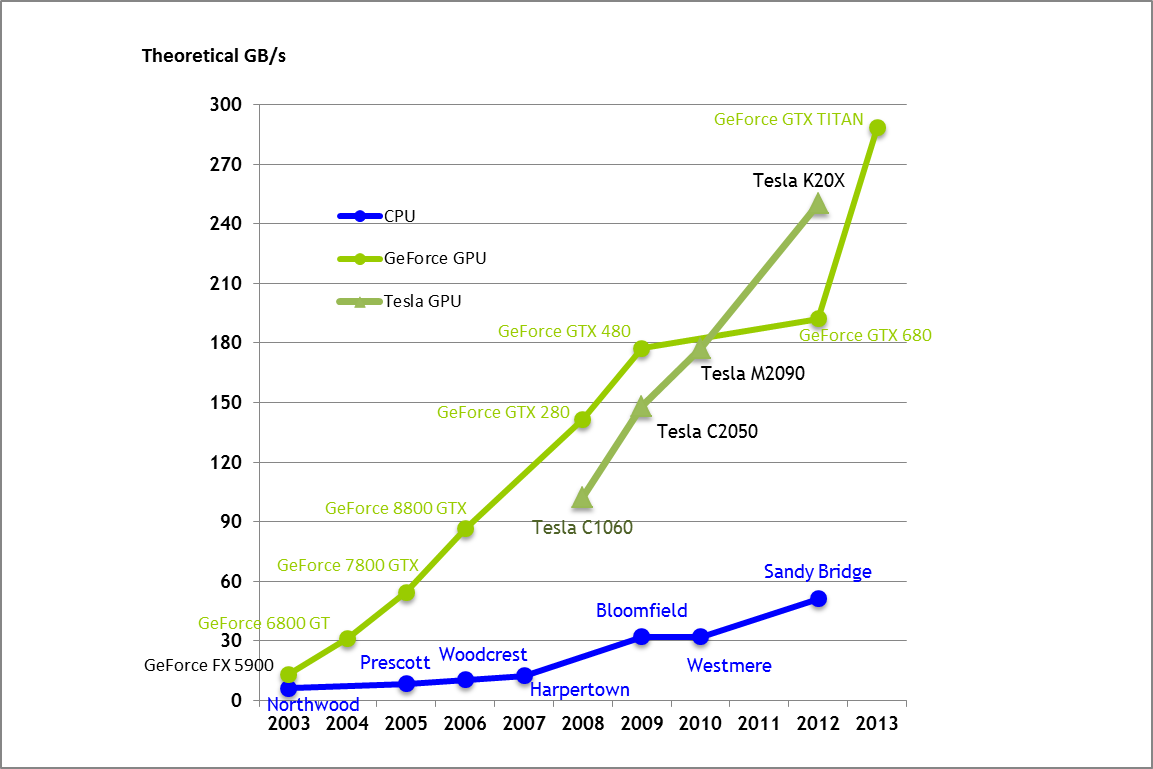
\includegraphics[width=0.9\textwidth]{gpu_content/nvidia_figures/memory-bandwidth.png}
\caption{Memory Bandwidth for the CPU and GPU (Image courtesy of NVidia \cite{CudaGuide2013})} 
\label{fig:memory-bandwidth}
\end{figure}

\begin{figure}
\centering
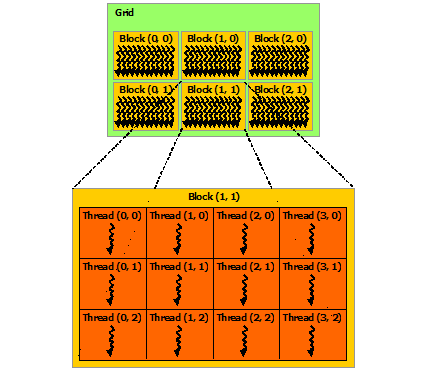
\includegraphics[width=0.7\textwidth]{gpu_content/nvidia_figures/grid-of-thread-blocks.png}
\caption{Grid of Thread Blocks (Image courtesy of NVidia \cite{CudaGuide2013})} 
\label{fig:grid-of-thread-blocks}
\end{figure}
